% ---------------------------------------------------------------------------
% axes.tex -- the experimental design: two orthogonal axes, four variants.
% Used at the head of the methodology.
% ---------------------------------------------------------------------------
\documentclass[border=8pt]{standalone}
% ---------------------------------------------------------------------------
% common.tex -- shared preamble for the hand-drawn TikZ diagrams of the thesis.
%
% Every diagram in this folder is a standalone document that inputs this file.
% Change a colour or a style here and it propagates to all figures at the next
% run of ./build.sh.
% ---------------------------------------------------------------------------

\usepackage[T1]{fontenc}
\usepackage{lmodern}
\usepackage{amsmath}
\usepackage{tikz}
\usetikzlibrary{arrows.meta, positioning, fit, backgrounds, calc, shapes.geometric}

% --- palette ---------------------------------------------------------------
\definecolor{diagInk}{RGB}{38,42,50}        % text
\definecolor{diagLine}{RGB}{118,128,142}    % neutral arrows and rules
\definecolor{diagGround}{RGB}{226,233,243}  % ground-and-solve fills
\definecolor{diagGroundEdge}{RGB}{ 96,132,178}
\definecolor{diagLazy}{RGB}{225,240,228}    % lazy fills
\definecolor{diagLazyEdge}{RGB}{ 76,147,100}
\definecolor{diagNeutral}{RGB}{242,242,244} % shared machinery
\definecolor{diagNeutralEdge}{RGB}{150,155,165}
\definecolor{diagAlert}{RGB}{252,232,229}   % the expensive artefact
\definecolor{diagAlertEdge}{RGB}{198, 88, 74}

% --- styles ----------------------------------------------------------------
\tikzset{
  % generic rounded box; the colour is given by one of the *fill styles below
  box/.style={
    draw, rounded corners=2.2pt, line width=0.7pt,
    align=center, inner xsep=7pt, inner ysep=6pt,
    font=\small, text=diagInk, minimum height=9.5mm
  },
  ground/.style={box, fill=diagGround, draw=diagGroundEdge},
  lazy/.style={box, fill=diagLazy,   draw=diagLazyEdge},
  neutral/.style={box, fill=diagNeutral, draw=diagNeutralEdge},
  alert/.style={box, fill=diagAlert,  draw=diagAlertEdge},
  % a box that holds code-like text
  mono/.style={font=\small\ttfamily},
  % arrows
  flow/.style={-{Stealth[length=2.6mm,width=2.0mm]}, draw=diagLine, line width=0.8pt},
  biflow/.style={{Stealth[length=2.6mm,width=2.0mm]}-{Stealth[length=2.6mm,width=2.0mm]},
                 draw=diagLine, line width=0.8pt},
  dashflow/.style={flow, dashed, dash pattern=on 2.6pt off 2.0pt},
  % small caption-like labels
  tag/.style={font=\scriptsize, text=diagInk, inner sep=2pt},
  lane/.style={font=\small\bfseries, text=diagInk},
  % the light band that groups a lane of the diagram
  band/.style={rounded corners=3pt, draw=none, inner sep=9pt},
}


\begin{document}
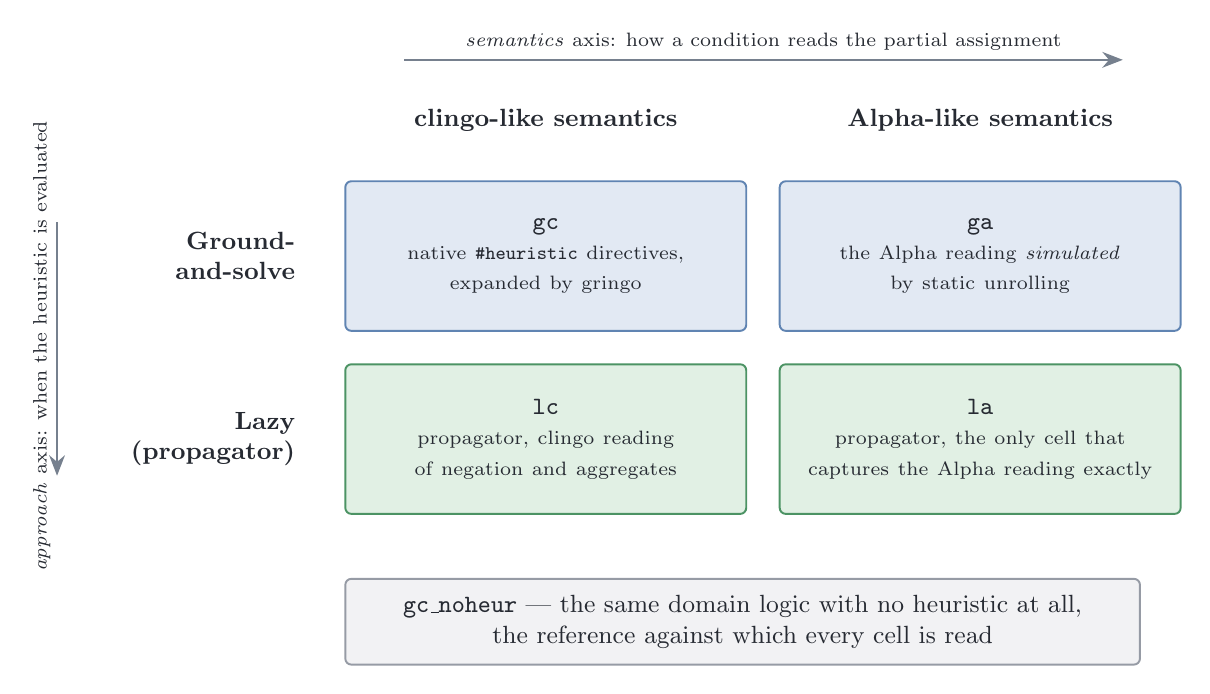
\begin{tikzpicture}

\def\cw{46mm}   % cell width
\def\ch{19mm}   % cell height
\def\gap{4mm}   % gap between cells

% ------------------------------- the four cells ----------------------------
\node[ground, text width=\cw, minimum height=\ch] (gc) at (0,0)
      {\textbf{\ttfamily gc}\\[3pt]{\scriptsize native \texttt{\#heuristic} directives,\\
       expanded by gringo}};
\node[ground, text width=\cw, minimum height=\ch, right=\gap of gc] (ga)
      {\textbf{\ttfamily ga}\\[3pt]{\scriptsize the Alpha reading \emph{simulated}\\
       by static unrolling}};
\node[lazy, text width=\cw, minimum height=\ch, below=\gap of gc] (lc)
      {\textbf{\ttfamily lc}\\[3pt]{\scriptsize propagator, clingo reading\\
       of negation and aggregates}};
\node[lazy, text width=\cw, minimum height=\ch, below=\gap of ga] (la)
      {\textbf{\ttfamily la}\\[3pt]{\scriptsize propagator, the only cell that\\
       captures the Alpha reading exactly}};

% ------------------------------- column headers ----------------------------
\node[lane, above=5mm of gc] (hc) {clingo-like semantics};
\node[lane, above=5mm of ga] (ha) {Alpha-like semantics};

% ------------------------------- row headers -------------------------------
\node[lane, text width=23mm, align=right, left=5mm of gc]  (rg) {Ground-\\and-solve};
\node[lane, text width=23mm, align=right, left=5mm of lc]  (rl) {Lazy\\(propagator)};

% ------------------------------- axis arrows -------------------------------
\draw[flow] ($(hc.north west)+(0,5mm)$) -- ($(ha.north east)+(0,5mm)$)
      node[tag, midway, above=1pt]
      {\emph{semantics} axis: how a condition reads the partial assignment};

\draw[flow] ($(rg.north west)+(-6mm,0)$) -- ($(rl.south west)+(-6mm,0)$)
      node[tag, midway, rotate=90, above=1pt]
      {\emph{approach} axis: when the heuristic is evaluated};

% ------------------------------- baseline ----------------------------------
\node[neutral, text width=96mm, below=8mm of lc.south west, anchor=north west]
      {\textbf{\ttfamily gc\_noheur} --- the same domain logic with no heuristic at
       all,\\ the reference against which every cell is read};

\end{tikzpicture}
\end{document}
